\documentclass[a4paper,12pt]{article}
\usepackage[utf8]{inputenc}
\usepackage[spanish]{babel}
\usepackage{color}
\usepackage{parskip}
\usepackage{graphicx}
\usepackage{multirow}
\usepackage{listings}
\usepackage{vmargin}
\graphicspath{ {imagenes/} }
\definecolor{mygreen}{rgb}{0,0.6,0}
\definecolor{lbcolor}{rgb}{0.9,0.9,0.9}
\usepackage{epstopdf}



\setpapersize{A4}
\setmargins{2.5cm}       % margen izquierdo
{1.5cm}                        % margen superior
{16.5cm}                      % anchura del texto
{23.42cm}                    % altura del texto
{10pt}                           % altura de los encabezados
{1cm}                           % espacio entre el texto y los encabezados
{0pt}                             % altura del pie de página
{2cm}     

\lstset{
backgroundcolor=\color{lbcolor},
    tabsize=4,    
%   rulecolor=,
    language=[GNU]C++,
        basicstyle=\tiny,
        aboveskip={1.5\baselineskip},
        columns=fixed,
        showstringspaces=false,
        extendedchars=false,
        breaklines=true,
        prebreak = \raisebox{0ex}[0ex][0ex]{\ensuremath{\hookleftarrow}},
        frame=single,
        showtabs=false,
        showspaces=false,
        showstringspaces=false,
        identifierstyle=\ttfamily,
        keywordstyle=\color[rgb]{0,0,1},
        commentstyle=\color[rgb]{0.026,0.112,0.095},
        stringstyle=\color{red},
        numberstyle=\color[rgb]{0.205, 0.142, 0.73},
%        \lstdefinestyle{C++}{language=C++,style=numbers}’.
}



\begin{document}

 \section{Problema}
 \subsection{Ejercicio 1}
 Una empresa de servicios guarda en una lista las tareas que debe realizar cada empleado. La estructura es la siguiente:
 \begin{itemize}
  \item Código Empleado
  \item Cantidad Tareas
  \item Cola de Tareas\par \smallskip
 \end{itemize}
 La cola de tareas tiene la siguiente estructura:
 \begin{itemize}
  \item Área solicitante
  \item Descripción \par \smallskip
 \end{itemize}
 Realizar procedimientos para este TDA que:
 \begin{itemize}
  \item Permita ingresar una nueva tarea en el empleado que tenga menos tareas.
  \item Permita ingresar una nueva tarea por código del empleado.
  \item Muestre el empleado con la mayor Cantidad de tareas y sus tareas pendientes.
  \item Muestre el empleado con la menor cantidad de tareas.
 \end{itemize}
 \subsection{Ejercico 2}
 En un hospital los pacientes sacan citas vía telefónica para ser atendidos en las diferentes especialidades que ofrece el hospital.
 Cada especialidad puede atender a 20 pacientes como máximo y la asignación de turnos es asignado por el tipo de gravedad.\par \smallskip
 Establezca el TDA Lista para cada especialidad y dentro de ellas, colas de prioridad. (La asignación de prioridad se debe hacer aleatoriamente).
 \begin{itemize}
  \item Asigne especialidades.
  \item Asigne pacientes a cada especialidad.
  \item Muestre los pacientes de una determinada especialidad.
  \item Lista la relación de todos los pacientes por especialidad.
 \end{itemize}
\twocolumn
 \section{Código}
 
 \subsection{Ejercicio 1}
 \subsubsection{ColaTareas.h}
  \lstinputlisting{cola.h}
 \subsubsection{ListaEmpleados.h}
  \lstinputlisting{lista.h}
 \subsubsection{main.h}
  \lstinputlisting{main.cpp}
  \newpage
 \subsection{Ejercicio 2}
 \subsubsection{ColaPrioridad.h}
  \lstinputlisting{colaP.h}
 \subsubsection{ListaEspecialidad.h}
  \lstinputlisting{listaEs.h}
 \subsubsection{main.h}
  \lstinputlisting{main2.cpp}
 \onecolumn

 \section{Ejemplos}
 \subsection{Ejercicio 1}
 \begin{figure}[h]
  \centering
  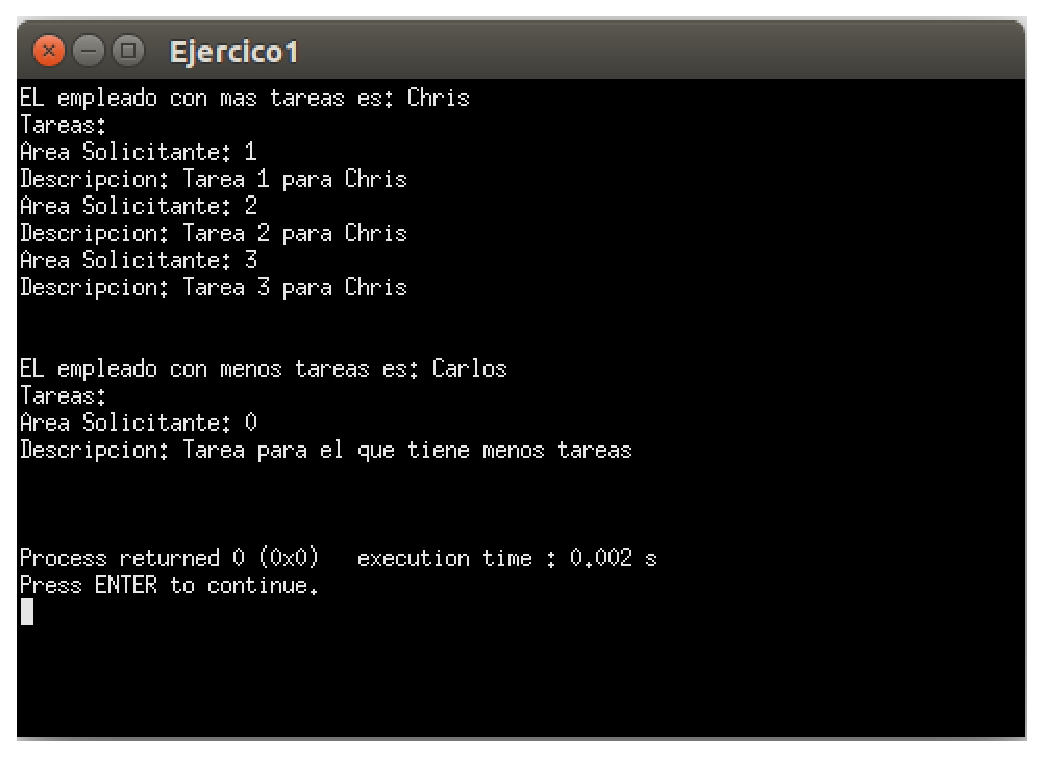
\includegraphics[scale = 0.5]{1.eps}
  \caption{Ejemplo Eje. 1}
 \end{figure}
 \subsection{Ejercicio 2}
 \begin{figure}[h]
  \centering
  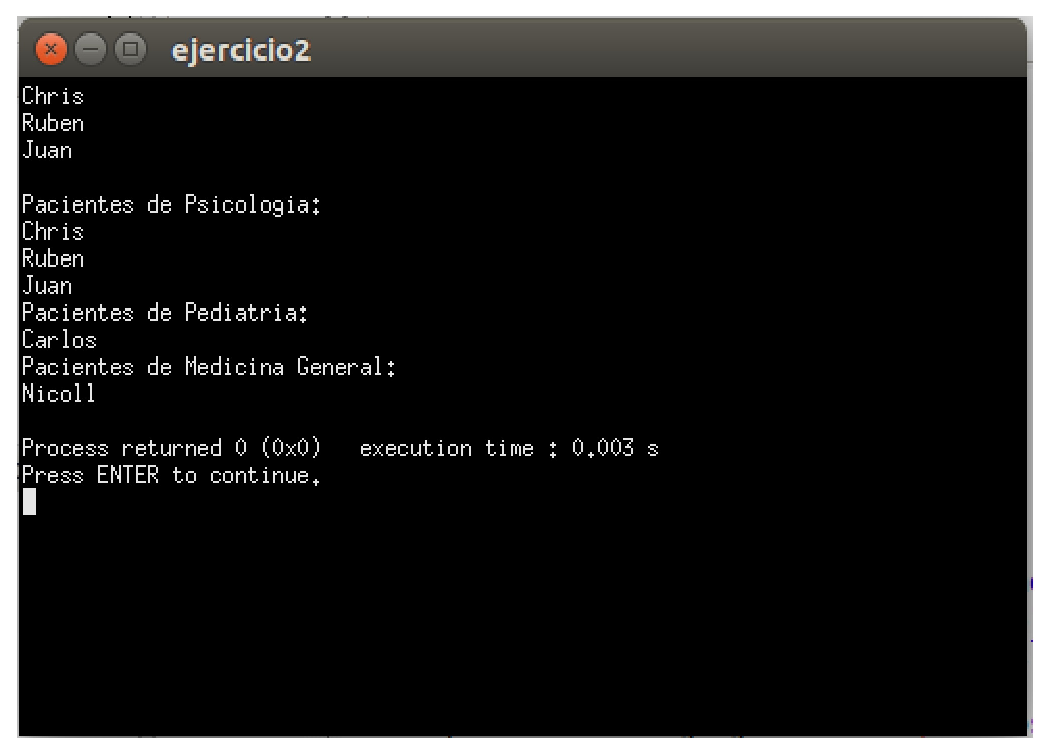
\includegraphics[scale = 0.5]{2.eps}
  \caption{Ejemplo Eje. 2}
 \end{figure}





 

 
\end{document}
